%!TEX root = ../../thesis.tex
\chapter{Bacteriophage Mosaicism}
\label{ch:phage}

\section{Introduction}
\label{phage:introduction}

Phages are microbial viruses which can infect bacteria, archaea, or single-celled eukaryotes.
By some measures, they are the most abundant and diverse class of organism on the planet.
It is estimated that there are $10^31$ extent bacteriophages \cite{Rohwer:2014vz}.\footnote{The estimate can be arrived at two independent ways: by assuming a total bacterial population size of $10^30$, and approximately ten phages per bacteria; or by the observation of a phage density of $10^6$ to $10^7$ per mL of seawater.}
This phage population completely turns over every few days -- an estimated infection rate of $10^23$ per second \cite{Suttle:2007cj}.

Phages play an essential role in natural ecosystems by regulating bacterial populations.
Steps have been taken towards harnessing this ability for productive use -- the FDA has approved several bacteriophage products designed to kill harmful bacteria in dairy and meat products \cite{Bren:2007wn}.
Also promising are potential phage therapies for treating pathogenic bacterial infections, although research in this direction is controversial \cite{Keen:2012du}.

Phages are classified based on lifestyle: virulent phages have a lytic life cycle and will infect a host, multiply, and exit the cell via lysis, killing the host organism. Temperate phages have a lysogenic life cycle and can remain within the host in a latent state, without disrupting host cellular function.
Phages can have a nucleic acid composition that is either double-stranded DNA (dsDNA), single-stranded DNA (ssDNA), double-stranded RNA (dsRNA), or single-stranded RNA (ssRNA).
Of these, dsDNA is by far the most common.
The typical genome length is on the order of $10^5$ bases, but can range from $10^3$ to $10^6$ bases.

The current bacteriophage taxonomy is compiled by the International Committee on Taxonomy of Viruses (ICTV) and is based on virus morphology, host range, lifestyle, and nucleic acid composition \cite{ICTV:2012}.
Table~\ref{phage:table:families} presents an overview of phage families defined by the ICTV.
There are two assigned orders and eighteen recognized families.
Fourteen families have dsDNA, two families have ssDNA, and two families have an RNA genome.
Because there is no single conserved gene across the phage population, there is currently no accepted way of constructing a molecular phage taxonomy.

% phage:table:families
\begin{table}[t]
    \caption{Phage families defined by the ICTV}
    \centering
    \scriptsize
    \begin{tabularx}{\textwidth}{lXlX}
    \toprule
    Order & Family & Morphology & Nucleic acid \\
    \midrule
    \multirow{3}{*}{\emph{Caudovirales}} & \emph{Myoviridae} & Nonenveloped, contractile tail & linear dsDNA \\
                                  & \emph{Siphoviridae} & Nonenveloped, noncontractile tail (long) & linear dsDNA \\
                                  & \emph{Podoviridae} & Nonenveloped, noncontractile tail (short) & linear dsDNA \\
    \midrule
    \multirow{2}{*}{\emph{Ligamenvirales}} & \emph{Lipothrixviridae} & Enveloped, rod-shaped & linear dsDNA \\
                                    & \emph{Rudiviridae} & Nonenveloped, rod-shaped & linear dsDNA \\
    \midrule
    \multirow{13}{*}{Unassigned} & \emph{Ampullaviridae} & Enveloped, bottle-shaped & linear dsDNA\\
                                 & \emph{Bicaudaviridae} & Nonenveloped, lemon-shaped & circular dsDNA \\
                                 & \emph{Clavaviridae}   & Nonenveloped, rod-shaped & circular dsDNA \\
                                 & \emph{Corticoviridae} & Nonenveloped, isometric & circular dsDNA \\
                                 & \emph{Cystoviridae}   & Enveloped, spherical & segmented dsRNA \\
                                 & \emph{Fuselloviridae} & Nonenveloped, lemon-shaped & circular dsDNA \\
                                 & \emph{Globuloviridae} & Enveloped, isometric & linear dsDNA \\
                                 & \emph{Guttaviridae}   & Nonenveloped, ovoid & circular dsDNA \\
                                 & \emph{Inoviridae}     & Nonenveloped, filamentous & circular ssDNA \\
                                 & \emph{Leviviridae}    & Nonenveloped, isometric & linear ssRNA \\
                                 & \emph{Microviridae}   & Nonenveloped, isometric & circular ssDNA \\
                                 & \emph{Plasmaviridae}  & Enveloped, pleomorph& circular dsDNA \\
                                 & \emph{Tectiviridae}   & Nonenveloped, isometric & linear dsDNA \\
    \bottomrule
    \end{tabularx}
    \label{phage:table:families}
\end{table}

It has long been known that phages are genetic mosaics subject to extremely high rates of reticulate genomic exchange \cite{Westmoreland:1969dd}.
The idea of mosaicism holds that phage species are composed of distinct modules that can be exchanged interchangeability within a population.
Exchange is facilitated within phages of the same host, thought certain phages are known to have broader host ranges.
The advent of full genome sequencing has reconfirmed this phenomenon and brought to bear questions about the applicability and interpretation of the ICTV taxonomy.
The ICTV taxonomy, based solely on morphology, has been shown to be inconsistent with the genomic data \cite{Lawrence:2002eg}.
As an example, in Figure~\ref{phage:fig:inconsistency} we show three different bacteriophage species: Enterobacteria phage HK97, Mycobacterium phage L5, and Enterobacteria phage P22.
HK97 is a Siphoviridae infecting \emph{E. coli}.
L5 is a Siphoviridae infecting \emph{M. smegmatis}.
P22 is a Podoviridae infecting \emph{S. enterica}.
HK97 and L5 belong to the Siphoviridae family comprised of long tail noncontracile phages.
P22 belongs to the Podoviridae family comprised of short tail phages.
Visually, it appears that HK97 and L5 should indeed be classified as distinct from P22.
However, genomic analysis indicates that HK97 and L5 share no gene content.
Despite belonging to different viral families, HK97 and P22 share 20\% gene content.
It is therefore clear that morphology and host range alone is not sufficient in representing phage relationships.

\begin{figure}
\centering
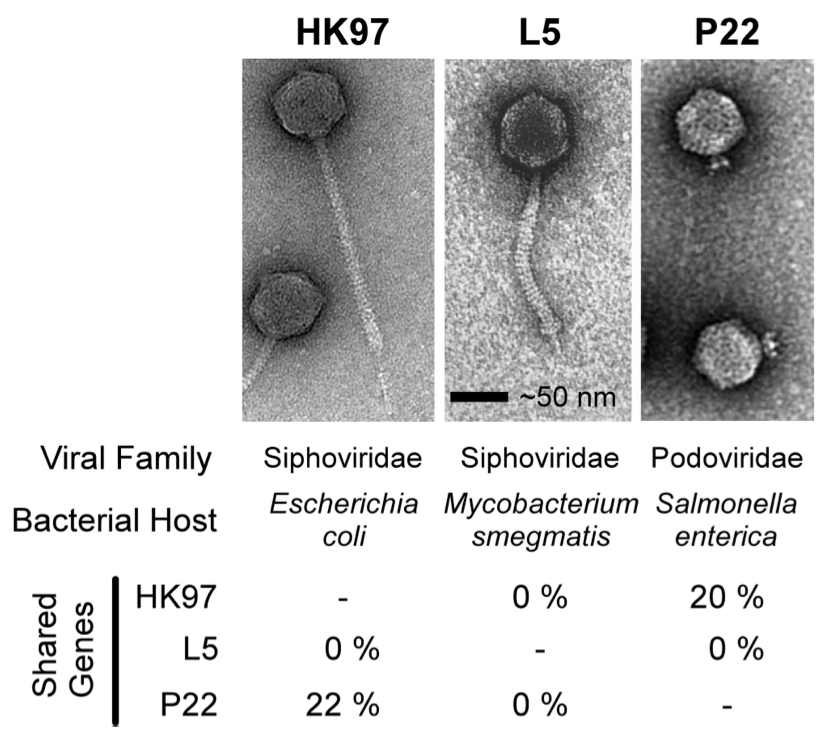
\includegraphics[width=.5\linewidth]{./fig/phage/LAWRENCE_phage_comparative.png}
\caption[Inconsistency of morphological classification in bacteriophage.]{Inconsistency of genomic and morphological approaches. HK97 and L5 are classified under same viral family, despite sharing no homologous genetic content. P22 on the other hand shares many genes. Figure adapted from \parencite{Lawrence:2002eg}.}
\label{phage:fig:inconsistency}
\end{figure}

Alternative representations of phage relationships have been proposed based on whole genome analysis.
For example, Rohwer and Edwards constructed a phage phylogenetic tree using differences in phage proteomes \cite{Rohwer:2002uo}.
Proux \emph{et al.} proposed a phylogenetic representation based on comparative analysis of head and tail sequences \cite{Proux:2002gj}.
However, these models still make the assumption of tree-like relationships.

In this chapter, we use approaches from topological data analysis to identify, measure, and represent reticulate evolution in a population of phage sequences.
This work is based on data collected by Lima-Mendez \emph{et al.} \cite{LimaMendez:2008ki} and Kristensen \emph{et al.} \cite{Kristensen:2013tt}.

First, we use persistent homology to characterize reticulation in phage genomes.
We find $H_0$ is largely inconsistent with existing phage taxonomies, and interpret $H_1$ as evidence for reticulate genetic exchange due to shared ecology and host range.
Second, we visualize phage relationships using Mapper, identifying clusters of phages with common gene content and host range.
The Mapper representations suggests an alternate way of representing phage relationships.

\section{Data}

We use data initially collected an analyzed in \cite{LimaMendez:2008ki}.
The data set consists of a collection of 306 bacteriophage genomes.
We show a summary of the data collected in Figure~\ref{phage:fig:phage_data_plot}.
Of the 306 genomes, 246 consist of dsDNA, 36 ssDNA, 12 dsRNA, and 8 ssRNA.
Four have unclassified nucleic acid material.
With respect to lifestyle, 146 are temperate and 72 are virulent.
Actinoplanes phage phiAsp2 is the single pseudotemperate phage, which means it largely maintains a temperate lifestyle but can occasionally enter a virulent state.
For 87 phages the lifestyle is unknown.
Taxonomically, the vast majority belong to order Caudovirales (221), which comprises Siphoviridae (117), Myoviridae (47), and Podoviridae (54). 
Order Ligamenviralies (4) comprises Lipothrixviriae (2) and Rudiviridae (2).
Unassigned families include Inoviridae (22), Cystoviridae (12), Gokushoviridae (8), and Microviridae (6).

\begin{figure}
\centering
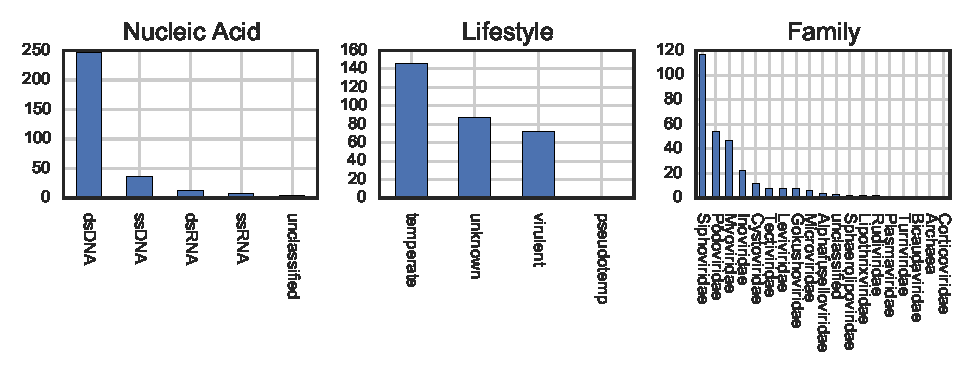
\includegraphics[]{./fig/phage/phage_data_plots.pdf}
\caption[Summary of phage data used in this analysis]{Summary of phage data used in this analysis. 306 bacteriophage genomes were included, as originally collected in \cite{LimaMendez:2008ki}. Here we show various annotations for the phage, including nucleic acid type, lifestyle, and taxonomic family (as defined by the ICTV). For some phage sequences this data is unknown.}
\label{phage:fig:phage_data_plot}
\end{figure}

The 306 bacteriophage genomes have been annotated and assigned genes.
There are 19,537 unique phage genes.
In the original study \cite{LimaMendez:2008ki}, these genes were clustered into 8,576 protein families using BlastP, which analyzes pairwise similarity of proteins.
Protein families share homology, which implies some degree of shared evolutionary ancestry.
Phages can then be represented as phyletic profiles in a binary protein family-space, indicating the presence or absence of a particular protein family.

\section{Measuring Phage Mosaicism with Persistent Homology}
\label{phage:ph}

First, we construct an appropriate metric space.
Because we have already transformed the phage genomes into phyletic profile representation, an evolutionary model is not explicitly necessary.
Instead, we follow \cite{LimaMendez:2008ki} and use a hypergeometric model as follows.
For two phages $A$ and $B$, let $a$ be the number of protein families in phage $A$, $b$ be the number of protein families in phage $B$, and $c$ be the number of protein families in common.
Let $n$ be the total number of protein families.
Then we can compute the p-value that the number of shared protein families $c$ is significant as
\begin{equation}
P_{AB} = \sum_{i=c}^{\min(a,b)} \frac{\binom{a}{i}\binom{n-a}{b-i}}{\binom{n}{b}}.
\end{equation}
To convert the p-values into a distance we take the log transform with small added noise,
\begin{equation}
d_{AB} = \log_{10}(P_{AB} + 10^{-10}) + 10.
\end{equation}
This yields a distance matrix $D$ with distances scaled between $0$ and $10$.
While this space does not explicitly reflect evolutionary divergence at a molecular level, it may be realistic at the protein level at which more complex types of genome evolution will have occurred.

To $D$ we now apply persistent homology.
We show the barcode diagrams in Figure~\ref{phage:fig:barcode}.
$H_0$ gives an initial classification.
We see that it is inconsistent with taxonomy.
Cycles in $H_1$ can be mapped to specific reticulation patterns.
These cycles may reflect shared environment.

\begin{figure}
\centering
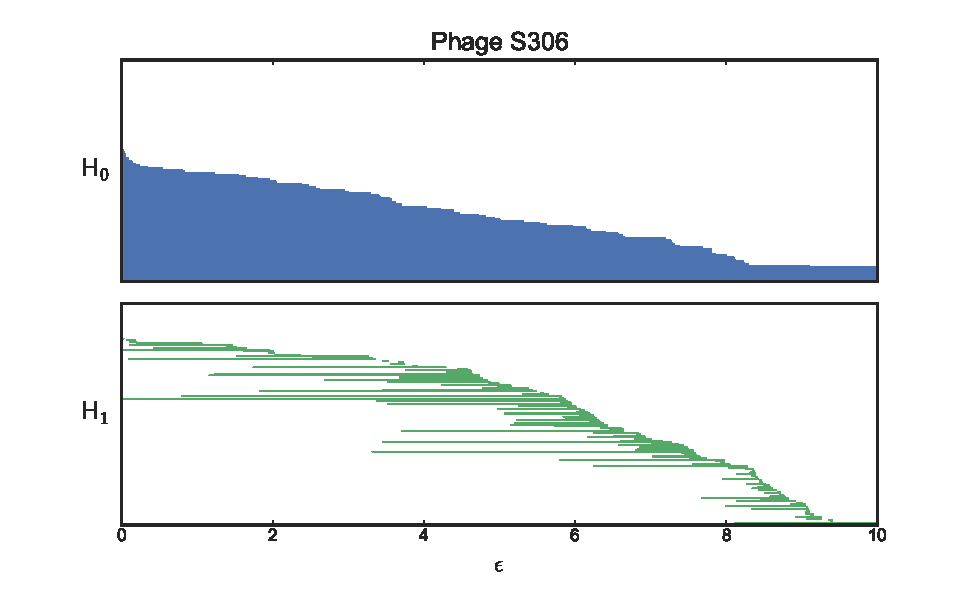
\includegraphics[]{./fig/phage/phage_s306_barcode.pdf}
\caption[Bacteriophage Barcode Diagram]{Bacteriophage Barcode Diagram using the S306 dataset.}
\label{phage:fig:barcode}
\end{figure}

\begin{figure}
\centering
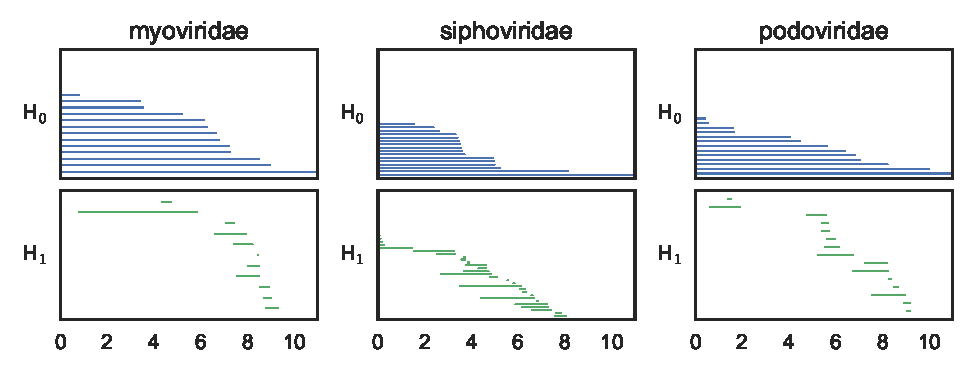
\includegraphics[]{./fig/phage/phage_s306_caudovirales_barcodes.pdf}
\caption[Caudovirales Barcode Diagrams]{Barcode Diagrams for Families of Order Caudovirales, including Siphoviridae, Myoviridae, and Podoviridae.}
\label{phage:fig:caudovirales_barcodes}
\end{figure}

In Figure~\ref{phage:fig:barcode} we show the barcode diagram.
We show the relationship of these bars within an existing phage taxonomy.
Extract multiscale patterns of reticulation.
Phage phylogeny taken from \cite{Glazko:2007dc}.

\section{Representing Phage Relationships with Mapper}
\label{phage:mapper}

We used Ayasdi Mapper to construct a network representation of the phage phyletic profiles.
The network was constructed using a Hamming metric and a 2D filter function.
First filter function was Metric PCA coord 1 with a resolution of 20 and a gain of 3.
Second filter function is metric PCA coord 2 with a resolution of 20 and a gain of 3.
The equalize setting was used for both filter functions.


We see several interesting things.
Using Ayasdi, we can identify gene enrichment in particular clusters.
We can also correlate with lifestyle and ecological properties.

One thing we can see is that the traditional classifications do not hold very well.

When we color by host, we see tighter correlation.
This suggests that a better classification would be based on host range.

\begin{figure}
\centering
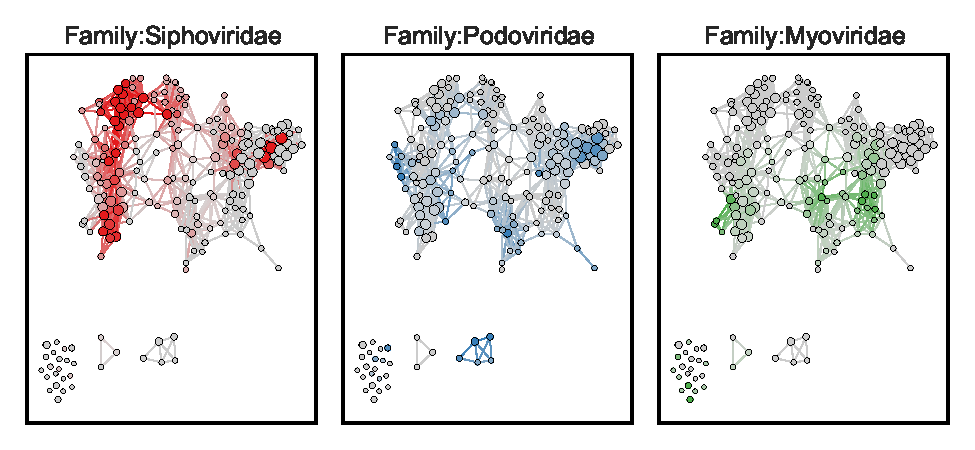
\includegraphics[]{{fig/phage/phage.s306.caudovirales_networks}.pdf}
\caption[Caudovirales Family Networks]{Caudovirales Family Networks}
\label{phage:fig:s306_caudovirales_networks}
\end{figure}

\begin{figure}
\centering
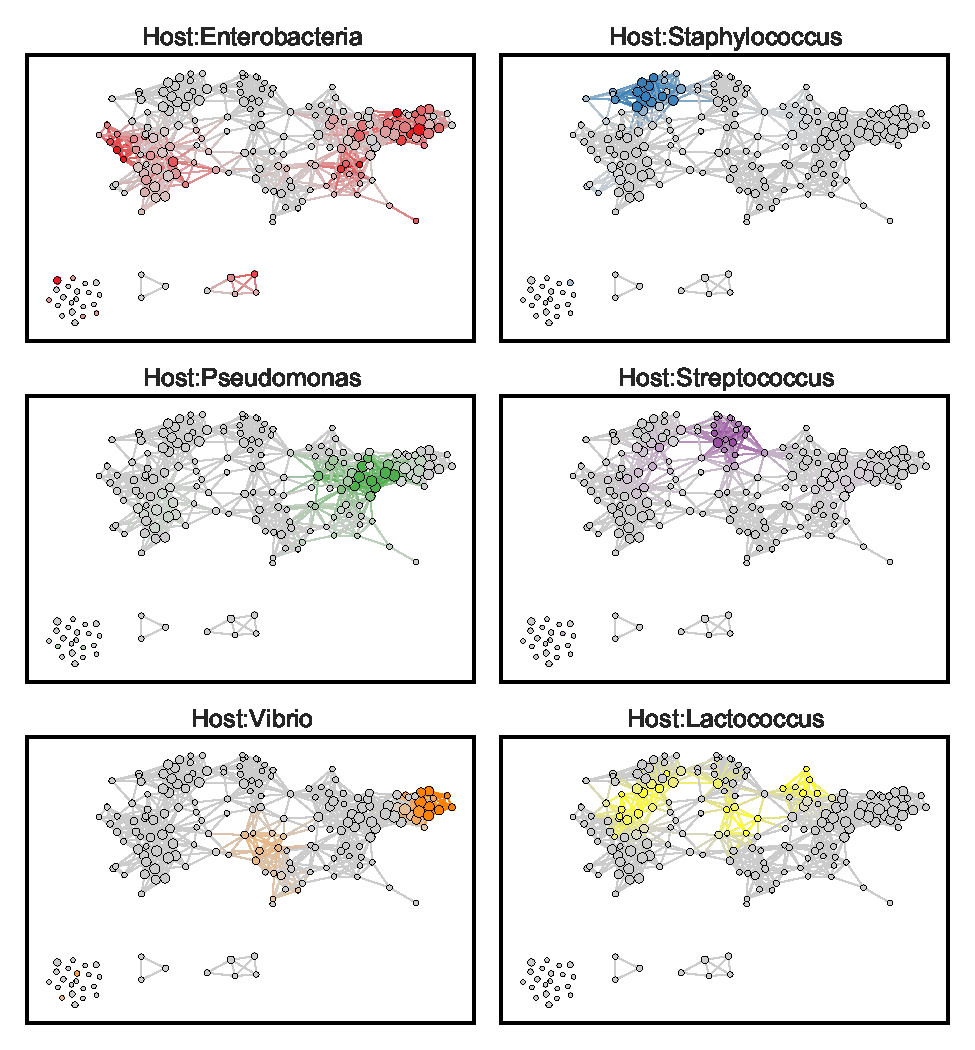
\includegraphics[]{{fig/phage/phage.s306.host_networks}.pdf}
\caption[Phage Host Networks]{Phage Host Network.}
\label{phage:fig:s306_host_networks}
\end{figure}

Finally, we clustered the network using the MCL graph clustering algorithm \cite{Enright:2002ep}, as implemented in XX.
The MCL algorithm takes two input parameters which control the coarseness of the clustering: an expand factor $e$ and an inflate factor $i$.
We set $e=5$ and $i=5$.
Ignoring the single nodes, this resulted in eleven clusters, as shown in Figure~\ref{phage:fig:s306_mcl_clustered_network}.

\begin{figure}
\centering
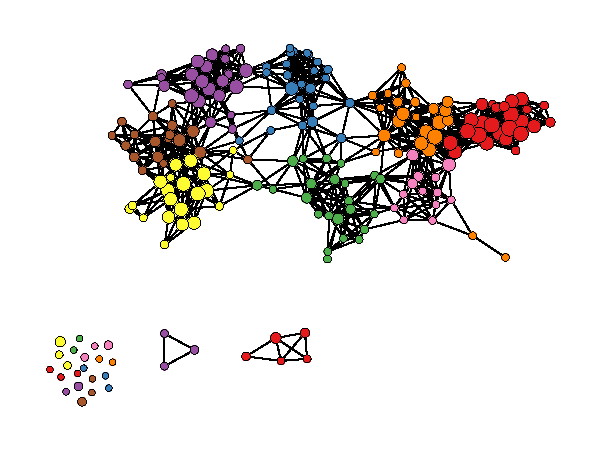
\includegraphics[]{{fig/phage/phage.s306.mcl_clustered_network}.pdf}
\caption[Phage Network with MCL Clustering]{Phage Network with MCL Clustering}
\label{phage:fig:s306_mcl_clustered_network}
\end{figure}

\section{Conclusions}
\label{phage:sec:conclusions}

In this chapter, we analyzed reticulate evolution in phages.
We demonstrated that phages have highly mosaic genomes.
We used approaches from topological data analysis to quantify reticulation and represent phage evolutionary relationships.
The Mapper representation allows for a systematic.